\chapter{Applicativo}

\section{Struttura}

L'interfaccia è stata realizzata utilizzando il linguaggio
di programmazione Python e la libreria PyQt versione 5.
PyQt è un'implementazione Python per Qt, un framework
multi-piattaforma per lo sviluppo di applicazioni grafiche.
Le sue principali caratteristiche sono la portabilità,
l'interoperabilità e la facilità di utilizzo.
Questo permette di poter impiegare lo stesso codice
su più sistemi operativi senza dover aggiungere
ulteriori livelli di complessità o l'utilizzo
di strumenti di virtualizzazioni.

Ai fini di testare l'applicativo sarebbe necessario
avere a disposizione un dispositivo ISCAN da poter collegare
al computer e vedere il comportamento dell'applicativo con
la sorgente video catturata.
Questo è ovviamente impratico per vari motivi,
dal dover impegnare lo strumento per lunghi periodi di tempo
alla necessità di avere un paziente che si stia sottoponendo
ad un esame in modo da avere un responso.
Per evitare queste problematiche, per fini puramente
dimostrativi, è stato realizzato anche uno script
per simulare la sorgente video dell'ISCAN, utilizzando
il software {\tt ffmpeg} e l'ecosistema {\tt V4L}.
{\tt V4L} è l'abbreviazione di {\it Video for Linux},
e permette la creazione di dispositivi video virtuali
su cui trasmettere un flusso video arbitrario, che verrà
percepito dal sistema operativo come un dispositivo video
reale, ad esempio una webcam o lo stesso ISCAN.

L'applicativo deve quindi principalmente essere in grado
di catturare un flusso video, in modo da poterne estrarre
i fotogrammi e ottenerne le predizioni dal modello.
Dalla predizione ottenuta bisognerà poi, tenendo conto
delle impostazioni scelte, ricreare l'immagine finale
da mostrare all'operatore.
Il modello in questo caso non viene istanziato direttamente
all'interno dell'applicazione, ma viene esposto come servizio
esterno con cui l'applicativo comunica tramite una API REST.
Le API REST sono un modo di comunicare con un servizio web
tramite richieste HTTP, la cui principale caratteristica
è la semplicità di utilizzo, e per questo molto popolare.
Questo tuttavia non significa che le immagini provenienti
dalla sorgente video escano dal computer e vengano
inviate in rete, in quanto il {\it server} che gestisce
tali richieste viene istanziato localmente e quindi
la comunicazione è limitata al computer su cui si sta
utilizzando l'applicativo.
Tuttavia sarebbe possibile estendere tale funzionalità in modo
da avere un servizio, esposto possibilmente su una rete locale,
che si occupa di gestire le richieste provenienti da più
applicativi, operazione che potrebbe essere interessante
per ridurre ulteriormente i costi o raccogliere ulteriori
dati per seguenti migliorie.

Il server che gestisce l'istanza del modello puo' essere
attivato tramite la libreria {\tt MMDeploy}\cite{mmdeploy},
facente parte dell'ecosistema {\tt OpenMMLab},
e che si occupa di semplificare la fase di {\it serving}
di modelli sviluppati con {\tt MMSeg} o altre librerie
facenti parte del progetto.
Come accennato, la libreria {\tt MMSeg} è costruita
al di sopra della libreria {\tt PyTorch}, che a sua volta
offre un suo software per il {\it serving} dei modelli
denominato {\tt torchserve}.
Tuttavia il formato impiegato da {\tt MMSeg} per esportare
i modelli, ovvero {\tt ONNX}, è diverso da quello di {\tt PyTorch},
e tale modello necessita quindi di essere convertito.
Una volta convertito il modello, {\tt MMDeploy} mette a
disposizione un'immagine {\tt Docker} per creare un'istanza
del modello sulla macchina, che a sua volta utilizzerà la
libreria {\tt torchserve}.
Uno script {\it ad-hoc} è stato creato per semplificare questa
fase, ma va fatto notare che una volta ottenuto un modello
soddisfacente è possibile derivare un'immagine derivata
da quella impiegata che contenga al suo interno il modello
in modo da semplificare drammaticamente questa fase.
I principali vantaggi dell'impiego di questa architettura
sono nuovamente la portabilità e la semplicità d'uso.
Avviata l'istanza sarà possibile inviare richieste HTTP
all'indirizzo preimpostato allegando l'immagine da analizzare,
da cui otterremo come rispsosta un'altra immagine contenente
la maschera predetta dal modello.

L'applicativo internamente utilizza un timer per catturare
i fotogrammi in modo da poterli inviare al modello.
Allo scadere del timer l'applicativo cattura un fotogramma
dalla sorgente video scelta e ne richiede la predizione che,
dopo essere stata visualizzata, farà ripartire il timer.
La frequenza con cui ciò accade è stata impostata 40
millisecondi, che corrisponde a circa 24 fotogrammi al secondo,
una frequenza video standard considerata sufficientemente fluida.
Tale scelta è dovuta a limitiazioni hardware, nel caso in cui
una precedente richiesta non sia stata ancora soddisfatta
non ne verranno inviate di nuove, ma è anche possibile, nel
momento in cui si disponga di hardware sufficientemente potente,
impostare il timer a valori più bassi o direttamente richiedere
che una nuova richiesta venga inviata non appena la precedente
è stata soddisfatta.


\section{Interfaccia}

L'interfaccia è stata sviluppata tenendo a mente gli obiettivi
funzionali preposti, dove ci si aspetta una fase di 
setup iniziale ridotta e conseguentemente un numero di interazioni
ridotte se non nulle al di fuori di guardare le predizioni
del modello.
All'avvio dell'applicazione viene mostrata una prima finestra
che richiede all'utente di selezionare la sorgente video
da utilizzare per catturare i fotogrammi.
Per catturare i fotogrammi è stata utilizzata la libreria
{\tt OpenCV} con la quale è possibile accedere a una sorgente
video tramite un ID numerico.
Questa prima fase dove si richiede di scegliere la sorgente
è dunque necessaria poiché non è possibile sapere a priori
quale sia la sorgente video da utilizzare, in quanto
più dispositivi video potrebbero essere collegati al computer
oppure a seconda dell'ordine in cui i sistemi operativi
assegnano l'ID alle sorgenti video questi potrebbero
essere diversi da quello che si aspetta.

\begin{figure}[H]
    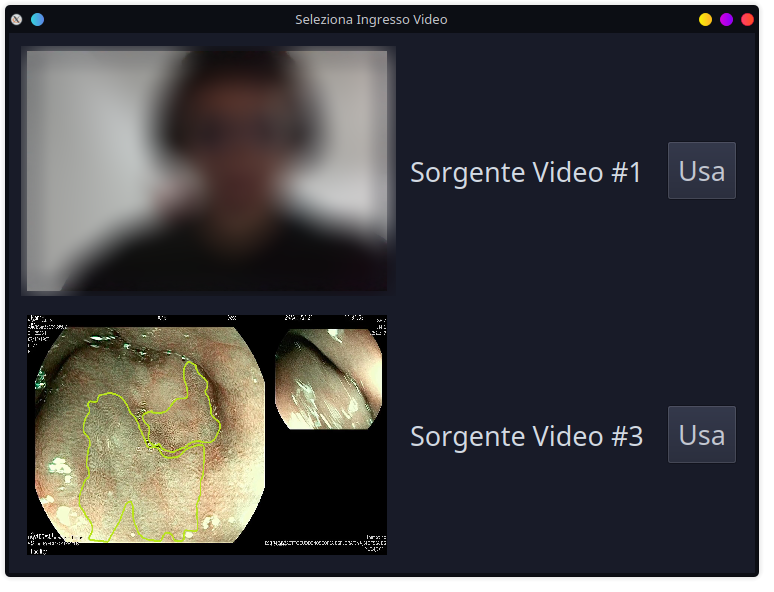
\includegraphics[width=0.9\textwidth]{./assets/app-splashscreen.png}
    \caption{\label{fig:app-splashscreen} Finestra selezione ingresso video}
\end{figure}

Per facilitare questa operazione viene quindi mostrato
accanto ad ogni possibile opzione una piccola anteprima
della sorgente video, in modo da poter scegliere quella
corretta.
Individuata l'entrata corretta, è sufficiente premere il
bottone "Usa" messo accanto, come visibile in 
figura \ref{fig:app-splashscreen}.

Questa fase esclude dal processo di selezione le sorgenti video
non valide o non disponibili.
Sempre in figura \ref{fig:app-splashscreen} infatti notiamo come
siano disponibili le sorgenti video 1 e 3, che corrispondono
ai dispositivi video 0 e 2, siano riportati in questa
finestra di selezione, mentre il dispositivo 1 e di conseguenza
la sorgente video 2 non è selezionabile.
Questo accade perché nella postazione di sviluppo dell'interfaccia
il dispositivo 1 è in realtà un'interfaccia virtuale del
dispositivo 0 e come tale non puo' essere impiegata per
l'acquisizione di immagini.

Selezionando una delle opzioni la finestra viene quindi chiusa
e si apre una seconda finestra che mostra il video selezionato
e dà l'accesso alle funzionalità dell'applicativo.
Da questo momento l'applicativo è gia in funzione
e al di sopra dell'uscita video vengono mostrare le predizioni
del modello.
Gli unici ulteriori controlli che l'utente puo' modificare a
suo piacimento sono degli {\it slider} che permettono di
regolare due parametri delle predizioni, che sono
l'opacità e lo spessore della maschera creata.
Questi due parametri sono stati resi modificabili in modo
da poter scegliere una combinazione che risulti
in maschere di predizioni visibili in modo chiaro e allo
stesso tempo che non coprano porzioni troppo elevate di
immagine o siano troppo distraenti.

A fini dimostrativi il colore per le predizioni è stato 
impostato  come un rosso acceso.
Tuttavia una scelta migliore è probabilmente quella di
utilizzare un colore che abbia più contrasto con quelli
che solitamente vengono visualizzati nelle immagini,
ovvero un verde acceso.
Non si è optato per questa decisione in quanto il video
generato per la dimostrazione utilizza le immagini
annotate e quindi creerebbe confusione, ma il cambio
del colore delle annotazione è una semplice modifica
di poco conto.
